\chapter{Integrity and attestation of distributed infrastructures (cloud, SDN, NFV, …)}

\section{Introduction}

\subsection{Typical distributed infrastructures}

\begin{figure}[h]
    \centering
    \shadowbox{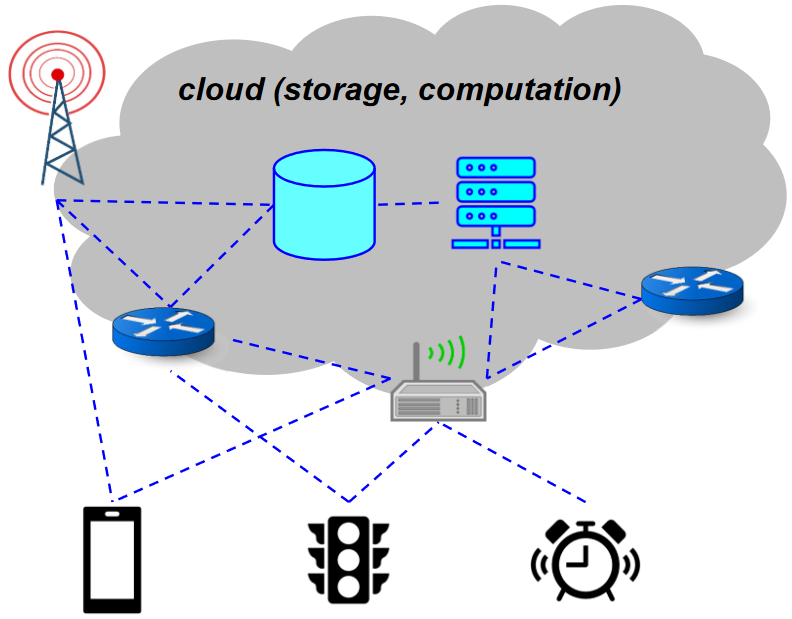
\includegraphics[width=0.4\textwidth]{img/dist-arch.png}}
    \caption{Distributed infrastructure}
    \label{fig:distributed_infrastructure}
\end{figure}


\begin{enumerate}[itemsep=0pt]
    \item Cloud computing (Server, Storage ...)
    \item edge devices (Router, Switch, \dots)
    \item IoT and personal devices (Smartphone, robot cleaner,  \dots)
\end{enumerate}

\subsection{Trend towards softwarization}
\begin{itemize}[itemsep=0pt]
    \item \textbf{SDN (Software-Defined Networking)}
    \item \textbf{... but also:}
    \begin{itemize}[itemsep=0pt]
        \item SDR, NFV, ...
        \item AI (!)
    \end{itemize}
    \item \textbf{As a consequence, more flexible but more vulnerable:}
    \begin{itemize}[itemsep=0pt]
        \item Software more prone to bugs than hardware
        \item Software updates
    \end{itemize}
\end{itemize}

\begin{quote}
- EASY (FAST, FLEXIBLE, ...) \\
- CHEAP \\
- SECURE \\
... PICK TWO!
\end{quote}

\subsubsection{Can I trust this infrastructure?}
A trustworthy infrastructure is defined as one that will behave in the expected way. However, several problems arise in achieving this trust:

\begin{itemize}[itemsep=0pt]
    \item Trust in the cloud provider(s)
    \item Trust in the network/edge provider(s)
    \item Low or no access control for edge- and end-devices
    \item Low-cost IoT devices (typically implying low security)
    \item Personal devices (typically managed by "ignorant" users)
\end{itemize}

If possible, the infrastructure should be protected to avoid or block attacks. Otherwise, it is essential to at least monitor the "state" of the system for early detection and possible reaction.

\subsection{Integrity}
\textbf{Hardware:}
\begin{itemize}[itemsep=0pt]
    \item Am I talking to the right (intended) node?
    \item Does it host the expected (physical) components?
\end{itemize}

\textbf{Software:}
\begin{itemize}[itemsep=0pt]
    \item Am I talking to the right (intended) software component?
    \item Is it correctly configured?
    \item Is the baseline software the expected one?
\end{itemize}

\section{TEE - Trusted Execution Environment}

\subsection{Trusted vs. Trustworthy}

\textbf{Trusted} refers to someone or something that you rely upon to not compromise your security. On the other hand, \textbf{Trustworthy} refers to someone or something that will not compromise your security. \\
\textit{Trusted} is about how you use something, while \textit{Trustworthy} is about whether it is inherently safe to use. \\
A \textbf{Trusted Execution Environment} is what you may choose to rely upon to execute sensitive tasks, such as running \textbf{Trusted Applications (TA)}. Ideally, this environment should be \textbf{Trustworthy} as well!

\subsection{TEE evolution}
The evolution of the \textbf{Trusted Execution Environment (TEE)} has gone through several significant milestones:

\begin{itemize}
    \item \textbf{Open Mobile Terminal Platform (now part of GSMA)} started the initiative.
    \item \textbf{2006}: Introduction of the \textbf{TR0 specifications}, outlining the basic security requirements.
    \item \textbf{2008}: Release of the \textbf{TR1 specifications}, which added the TEE layer on top of TR0.
    \item \textbf{2010}: \textbf{GlobalPlatform} was launched to define interfaces and provide certifications, becoming the de-facto standardization body for TEEs.
    \item \textbf{2012}:
    \begin{itemize}
        \item \textbf{ARM}, \textbf{Gemalto}, and \textbf{G+D} formed \textbf{Trustonic}, aiming to create an open TEE.
        \item \textbf{GlobalPlatform} and the \textbf{Trusted Computer Group (TCG)} created a joint working group to focus on TEE specifications and its integration with the \textbf{Trusted Platform Module (TPM)}.
    \end{itemize}
\end{itemize}
The first major business case for the Trusted Execution Environment (TEE) was Netflix's high-resolution content on smartphones and tablets. Following this, TEE's application rapidly expanded into various sectors, including financial services, enterprise solutions, government security, automotive industries, and the Internet of Things (IoT)

\subsection{TEE and REE}
\begin{figure}[h]
    \centering
    \shadowbox{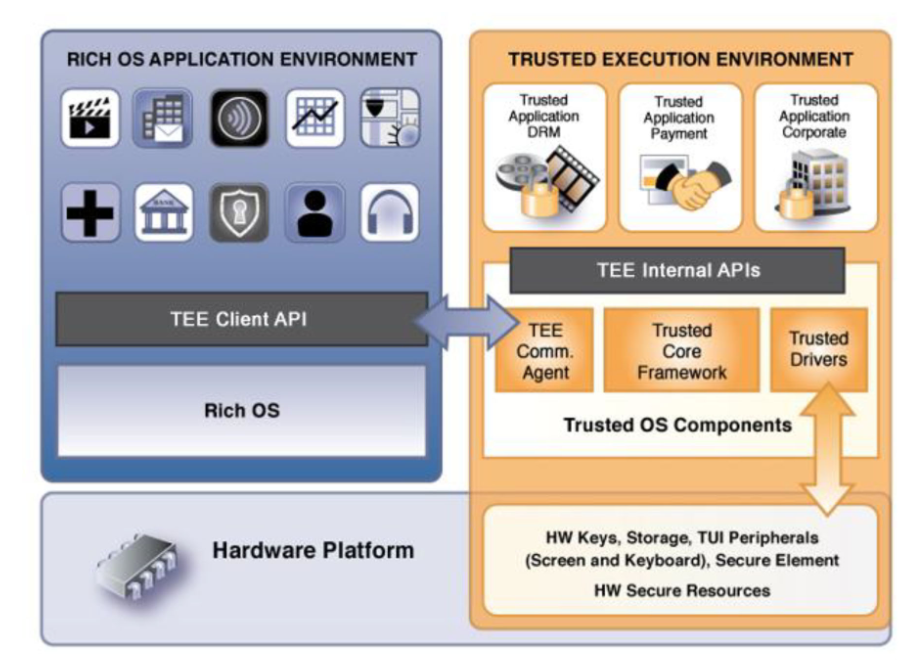
\includegraphics[width=0.4\textwidth]{img/tee-ree.png}}
    \caption{TEE and REE}
    \label{fig:tee_ree}
\end{figure}

\subsection{Some key points}
\textbf{Trusted Execution Environment (TEE)} is currently a hot topic in the realm of \textit{confidential computing}, which is promoted by the \textbf{Confidential Computing Consortium (CCC)}. One of the key objectives of TEE is the protection of \textbf{data in use}, ensuring that no unauthorized entity can read or write this data, and it is processed only by an authorized application. This is in contrast to various cryptographic techniques used to protect \textit{data at rest} and \textit{data in motion}. \bigskip

A critical component of TEE is the \textbf{Root of Trust (RoT)}, an element whose misbehavior cannot be detected during runtime. It is essential that the RoT be both \textit{trusted} and \textit{trustworthy}. The RoT is part of the \textbf{Trusted Computing Base (TCB)}, which includes all hardware, firmware, and software components that are crucial to the system's security. Any vulnerability within the TCB could potentially jeopardize the security of the entire system.

\subsection{Intel IPT}

\textbf{Intel Identity Protection Technology (IPT)} is a security feature that runs a Java applet on a separate CPU. The \textbf{Management Engine} is part of the chipset, meaning it is bound to the physical hardware. This setup enables a variety of secure applications, including:

\begin{itemize}
    \item Key generation and storage (integrated with Windows Cryptographic API)
    \item One-Time Password (OTP) generation (e.g., VASCO MYDIGIPASS.COM)
    \item Secure PIN entry
    \item \begin{itemize}
        \item These features are made possible because the chipset also manages video
    \end{itemize}
\end{itemize}

\subsection{ARM TrustZone}

\textbf{ARM TrustZone} extends CPU buses to a "33rd bit," which signals whether the CPU is in secure mode or not. This signal is exposed outside of the CPU, enabling the use of secure peripherals and secure RAM. 

Key characteristics include:
\begin{itemize}
    \item The system is open and well-documented.
    \item But, it only allows for \textit{one} secure enclave.
    \item ARM is working on adding a \textit{third mode} to enhance its capabilities.
\end{itemize}

Additionally, there is potential for an indicator to signal the current mode the CPU is operating in.

\subsection{Trustonic}

\subsection{Intel SGX}

\subsection{Keystone}

\subsubsection{Motivation for Keystone}

\subsubsection{Keystone architecture}

\subsubsection{Keystone: further reading}


\section{Trusted computing and remote attestation}

\subsection{Baseline computer system protection}

\subsection{Rootkits}


\subsection{Software to protect software?}


\subsection{Firmware self-protection (SW root-of-trust)}

\subsubsection{HW root-of-trust for firmware protection}

\subsection{Boot Types}

\subsubsection{Windows boot protection}


\section{What is Trusted Computing?}

\subsection{Trusted Computing Base (TCB)}

\subsection{Root of Trust (RoT)}


\subsection{Chain of trust}


\section{Trusted Platform Module (TPM) overview}

\subsection{TPM features}

\subsection{TPM-1.2}

\subsection{TPM-2.0}

\subsubsection{Implementation of TPM-2.0}

\subsubsection{TPM-2.0 three hierarchies}


\subsection{Using a TPM for securely storing data}

\subsection{TPM objects}

\subsection{TPM object's area}

\subsection{TPM Platform Configuration Register (PCR)}